%%%%%%%%%%%%%%%%%%%%%%%%%%%%%%%%%%%%%%%%%%%%%%%%%%%%%%%%%%%%%%%%%%%%%
%
% cours Intro à l'optimisation pour le machine learning
%
%%%%%%%%%%%%%%%%%%%%%%%%%%%%%%%%%%%%%%%%%%%%%%%%%%%%%%%%%%%%%%%%%%%%%

\documentclass[12pt]{beamer}
\usepackage[utf8]{inputenc}
\usepackage{amsmath}
\usepackage{amsfonts}
\usepackage{amssymb}
\usepackage{graphicx}
\graphicspath{{figures/}}
%\usepackage{beamerthemesplit}
%\usepackage{beamerthemeshadow} 
\usepackage{color}
\usepackage{hyperref}
\usepackage{xspace}
\usepackage{xifthen}
\usepackage{multicol}
\usepackage{mathtools}
\usepackage{algorithm,algorithmic}
\usepackage{dsfont}
%
% these 2 next needed for mathbb greek letters
\usepackage{breqn} 
\usepackage[bbgreekl]{mathbbol}
%
\usepackage{bbm} % this one is needed for the indicator
%
\usepackage{tikz}
\usetikzlibrary{calc,shapes,arrows,positioning}
%
% handwritten font
\newcommand*{\hwfont}{\fontfamily{qzc}\selectfont}
\DeclareTextFontCommand{\texthw}{\hwfont}

% custom commands in sty file, for easier writting and change of notations
\usepackage{my_notations}

\usetheme{Madrid}
\usecolortheme{beaver}

%%%%%%%%%%%%%%%%%%%%%%%%%%%%%%%%%%%%%%%%%%%%%%%%%%%%%%%%%%%%%%%%%%%%%
\begin{document}
\title
[~Optimisation pour le machine learning
%\hspace{0.5cm}
%\insertframenumber/\inserttotalframenumber
]
{Introduction à l'optimisation pour le machine learning}
\author
[Le Riche et al.]
{\large Rodolphe Le Riche$^1$, Dédji Brian Whannou$^2$, Espéran Padonou$^3$} 
\institute[CNRS/fondat. Vallet]{
$^1$ CNRS LIMOS at Mines Saint-Etienne, France \\
$^2$ KPMG France \\
$^3$ Fondation Vallet
} 
\date[Juillet 2021]{Juillet 2021 \\
Ecole d'Eté en Intelligence Artificielle \\
fondation Vallet\\
Cotonou, Bénin} 
\begin{frame}
\titlepage
\end{frame}

\section{Introduction}
\subsection{Objectifs, remerciements}

%%%%%%%%%%%%%%%%%%%%%%%%%%%%%%%%%%%%%%%%%%%%%%%%%%%%%%%%%%%%%%%%%%
\begin{frame}%[allowframebreaks]
\frametitle{Plan du cours} 
%\begin{multicols}{2}
\begin{center} \textbf{Introduction à l'optimisation pour le machine learning} \end{center}
\tableofcontents[currentsection]
%\end{multicols}
\end{frame}

%%%%%%%%%%%%%%%%%%%%%%%%%%%%%%%%%%%%%%%%%%%%%%%%%%%%%%%%%%%%%%%%%
\begin{frame}
\frametitle{Objectifs du cours}
\begin{itemize}
\item Donner des bases pour l'optimisation numérique
\item en faisant le lien avec le machine learning
\item pour un public de bac+1
\item avec quelques exemples de programmes en R/python.
\item Limites: les algorithmes ne seront pas exactement ceux utilisés en pratique pour le deep learning, mais les principaux concepts y seront.
\end{itemize}
\end{frame}

%%%%%%%%%%%%%%%%%%%%%%%%%%%%%%%%%%%%%%%%%%%%%%%%%%%%%%%%%%%%%%%%%
\begin{frame}
\frametitle{Bibliographie du cours}
Ce cours doit beaucoup à
\begin{itemize}
\item \cite{minoux2008programmation} : un classique sur l'optimisation, écrit avant l'avènement du machine learning mais une vraie base (niveau bac+3)
\item \cite{ravikumar17} : présentation détaillée des algorithmes d'optimisation utiles en machine learning (niveau bac+3)
\item \cite{bishop2006pattern} : un excellent livre d'introduction au machine learning avec quelques commentaires sur l'optimisation (niveau bac+3)
\item \cite{schmidt2007fast} : techniques pour la régularisation L1 (article de recherche)
\item \cite{sun2019optimization} : panorama des méthodes d'optimisation pour les réseaux de neurones, rétro-propagation de gradient (article de recherche)
\end{itemize}
Nous en simplifierons le contenu et emprunterons des illustrations.
\end{frame}

\subsection{Formulation d'un problème d'optimisation}

%%%%%%%%%%%%%%%%%%%%%%%%%%%%%%%%%%%%%%%%%%%%%%%%%%%%%%%%%%%%%%%%%
\begin{frame}
\frametitle{Optimisation = formalisation de la décision}
L'optimisation est une\footnote{non unique, contestable par rapport à l'humain et la vie} formalisation mathématique de la décision
\vskip\baselineskip
\mbox{
\begin{minipage}[c]{0.3\textwidth}

\includegraphics[width=\textwidth]{decision-clipart.jpg}
\end{minipage}
\begin{minipage}[c]{0.7\textwidth}
\begin{equation*}
\min_{x \in \mathcal S} f(x)
\end{equation*}
\begin{itemize}
\item $x$ vecteur des paramètres de la décision~: dimensions, somme investie, réglage d'une machine/code, \ldots
\item $f(x)$~: coût de la décision $x$
\item $\mathcal S$~: ensemble des valeurs possibles de $x$, espace de recherche
\end{itemize}
\end{minipage}
} % end mbox
\end{frame}

%%%%%%%%%%%%%%%%%%%%%%%%%%%%%%%%%%%%%%%%%%%%%%%%%%%%%%%%%%%%%%%%%
\begin{frame}
\frametitle{Exemple d'optimisation: identification d'un modèle}
\begin{center}
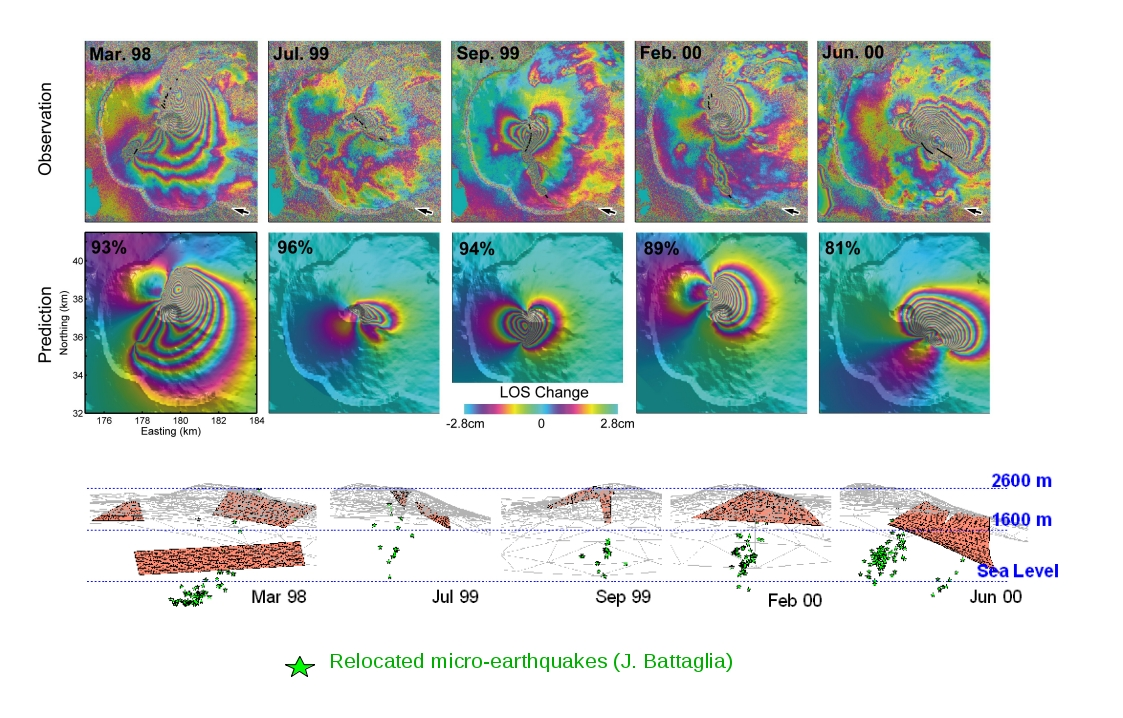
\includegraphics[width=0.7\textwidth]{piton_fournaise.jpg}
\end{center}
\end{frame}
{\small extrait de \cite{fukushima2010evolution}}
\subsection{Exemple en machine learning}

\section{Descente de gradient}
%%%%%%%%%%%%%%%%%%%%%%%%%%%%%%%%%%%%%%%%%%%%%%%%%%%%%%%%%%%%%%%%%%
\begin{frame}%[allowframebreaks]
\frametitle{Plan du cours} 
%\begin{multicols}{2}
\begin{center} \textbf{Introduction à l'optimisation pour le machine learning} \end{center}
\tableofcontents[currentsection]
%\end{multicols}
\end{frame}
\subsection{Algorithme}
\subsection{Application aux réseaux de neurones: la rétropropagation de gradient}

\section{Accélarations du gradient}
%%%%%%%%%%%%%%%%%%%%%%%%%%%%%%%%%%%%%%%%%%%%%%%%%%%%%%%%%%%%%%%%%%
\begin{frame}%[allowframebreaks]
\frametitle{Plan du cours} 
%\begin{multicols}{2}
\begin{center} \textbf{Introduction à l'optimisation pour le machine learning} \end{center}
\tableofcontents[currentsection]
%\end{multicols}
\end{frame}

\section{Prise en compte des contraintes d'optimisation}
%%%%%%%%%%%%%%%%%%%%%%%%%%%%%%%%%%%%%%%%%%%%%%%%%%%%%%%%%%%%%%%%%%
\begin{frame}%[allowframebreaks]
\frametitle{Plan du cours} 
%\begin{multicols}{2}
\begin{center} \textbf{Introduction à l'optimisation pour le machine learning} \end{center}
\tableofcontents[currentsection]
%\end{multicols}
\end{frame}

\section{Conclusions}

%%%%%%%%%%%%%%%%%%%%%%%%%%%%%%%%%%%%%%%%%%%%%%%%%%%%%%%%%%%%%%%%%
\begin{frame}
\frametitle{Conclusions}
\begin{itemize}
\item L'optimisation numérique est une technique fondamentale associée à la décision optimale et à la modélisation statistique (machine learning).
\item Avec l'enthousiasme autour du machine learning, de nombreux algorithmes ont été conçus que nous n'avons pas couverts ici: l'optimisation bayésienne (Bayesian optimization) pour le réglage des hyper-paramètres (paramètres de régularisation, nombre de couches du réseau de neurone, type de neurones, paramètres de l'algorithme d'optimisation des poids).
\end{itemize}
\end{frame}

\section{Bibliography}

%=======================================================================================
\begin{frame}[allowframebreaks]
\frametitle{References}
\scriptsize
%\vspace{-1.cm}
%\setbeamertemplate{bibliography item}{[\theenumiv]} % to have numbers in biblio with beamer
%   \bibliographystyle{plain}
   \bibliographystyle{apalike}
   \bibliography{biblio}
\end{frame}

\end{document}
